\chapter{Stand der Technik}

In diesem Kapitel werden kurz einige verwandte Arbeiten vorgestellt, die eine Grundlage für diese Thesis bildeten.

\section{Grundmodell}

Craig Reynolds hat als einer der ersten versucht einen Schwarm mit einfachen Mitteln darzustellen. Er modellierte einen Schwarm mit Vögel im 3dim-Raum. Dazu stellte er 3 Regeln auf mit denen ein Schwarm sein Verhalten berechnet:
\begin{itemize}
\item Separation: steer to avoid crowding local flockmates
alignment diagram 	
\item Alignment: steer towards the average heading of local flockmates
cohesion diagram 	
\item Cohesion: steer to move toward the average position of local flockmates 
\end{itemize}
Auf dieser Grundlage wurde in den nachfolgenden Jahren viel Forschung betrieben und das Verhalten der heutigen Roboter-Schwärme ausgearbeitet die sich an der Natur orienten.\cite{CraigReynolds_Boids}

\section{Erweiterung des Modells}
Vicsek hat in seinen weiteren Forschungen das Modell seiner Vogel-Schwärme erweitert. In einer seiner Veröffentlichungen erweitert er das Modell der schwarmgetriebenen Partikel dahingehend, dass nicht nur die Ausrichung der anderen Roboter entscheidend ist, sondern auch deren Geschwindigkeit.
Dabei konnten neue Muster in den Schwärmen erkannt werden, die in Abhängigkeit der Variable \textit{s} standen. \textit{s} ist dabei der Wert, der angibt, wie sehr sich Einheiten an der Geschwindigkeit anderer Einheiten orientieren im Intervall von [0,1]. Ab einem Wert von 0.59 stieg die Bindung des Schwarms rapide an, ähnlich wie man es bisher bei einem kritischen Wert des freien Willens kannte.\cite{VicsekAcceleration} 

\section{Informierte Anführer}

Da ein Schwarm nicht direkt gelenkt werden kann, werden mittel gesucht ihn mit seinen eigenen Mitteln zu lenken. Ein Versuch dabei ist das Vorgehen mit 'Informierten Anführern'. In dem Paper wurden einige Roboter über das Ziel informiert, zu dem der Schwarm gelenkt werden soll. Diese informierten Anführer lenkten daraufhin den Schwarm dadurch, dass sie eine konstante (und einigermaßen gleiche) Ausrichtung hatten, an der sich die Roboter während ihres normalen Schwarmverhaltens orientierten.\cite{RobotLeader}

\newpage\section{Kilobots}

%\begin{wrapfigure}{r}{\pictureWidthBig}
%	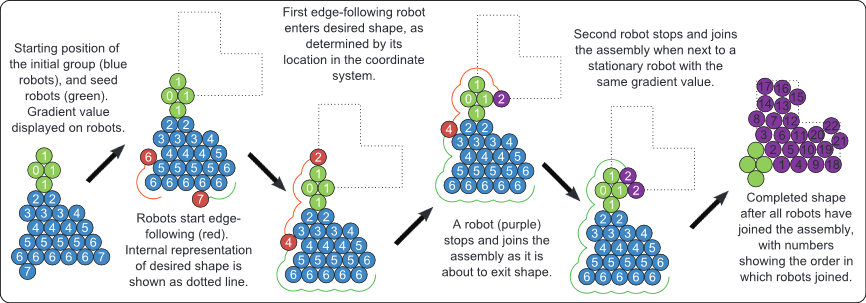
\includegraphics[width=\pictureWidthBig,keepaspectratio]{graphics/Kilobot.png}
%	\caption{Struktur-Erstellung mit Kilobots}
%	\label{pic:Kilobot}
%\end{wrapfigure}

In einem Paper von Harvard wird demonstriert, wie Roboter ('Kilobots') eine vordefinierte Fläche eigenständig ausfüllen. Dafür wurde ein "Bild" genommen, das den Robotern dient um die Fläche zu erkennen. Die Roboter kommunizieren nur wenig miteinander. Sie sind in der Lage ein Koordinatensystem aufzuspannen und ihre Position innerhalb dessen zu erkennen. Außerdem können sie sich selbst einen 'Gradienten', eine Art numerische Einstufung zuteilen und diese mit anderen mitteilen. Als letzte Fähigkeit können sie einer Kante folgen. Sie sind damit in der Lage den Rand eines bereits bestehenden Roboter-Haufens entlang zu gehen ohne mit ihnen zusammenzustoßen.

\begin{figure}[h]
	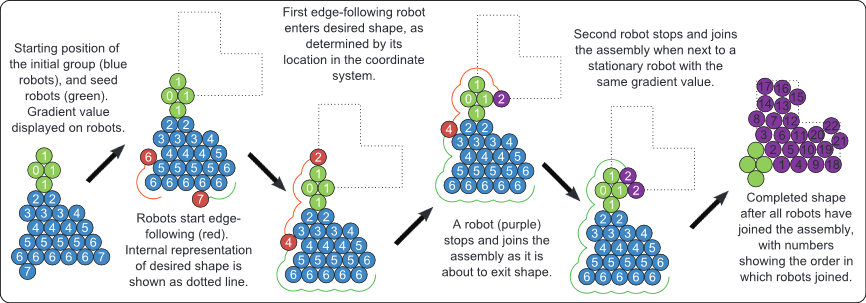
\includegraphics[width=\textwidth,keepaspectratio]{graphics/Kilobot.png}
	\caption{Struktur-Erstellung mit Kilobots}
	\label{pic:Kilobot}
\end{figure}

Gestartet wird der Algorithmus mit einem "Seed", einem Roboter der der die Koordinate (0,0) bildet. Die anderen Roboter kommen nach und nach dazu und hangeln sich die bereits stehenden Roboter entlang. Sein Gradient wird dabei ständig angepasst. Dieser wird auf den kleinsten Gradienten in seiner Umgebung + 1 gesetzt, während der Seed immer auf 0 bleibt.
Verlässt ein Roboter das Bild oder stößt auf einen anderen Roboter mit dem selben Gradienten, bleibt dieser stehen.\cite{Kilobot} Der Algorithmus ist in \autoref{pic:Kilobot} zu sehen.

\section{Transport}

Am \textit{Intelligent Robotics Research Centre, Monash University} beschäftigte man sich damit, wie Bienen andere tote Bienen aus einem Nest befördern. Bienen sondern bei ihrem Tod ein Pheromon ab, dass andere Bienen dazu veranlasst, den Leichnam aus dem Bau zu stoßen.

\begin{wrapfigure}{r}{\pictureWidthBig}
	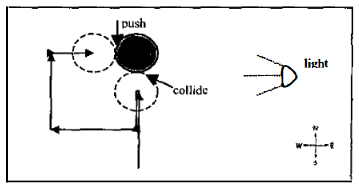
\includegraphics[width=\pictureWidthBig,keepaspectratio]{graphics/PaperBienen.png}
	\caption{Struktur-Erstellung mit Bausteinen}
	\label{pic:StrukturenKloetze}
\end{wrapfigure}

Im Experiment wurden Roboter vorgestellt die mit einem Gas-Sensor ausgestattet sind und ein kleiner, spezieller Roboter, der in der Lage ist eben solches Gas auszustoßen. Die Roboter suchen permanent nach der Quelle des Gases und fahren dabei in Kreisen, um die Quelle zu lokalisieren. Ist die Quelle gefunden und angestoßen, positionieren sie sich so, dass die Quelle zwischen ihnen und einer Lichtquelle steht. Anschließend wird die Quelle geschoben und eine erneute Suche nach der Quelle gestartet, da diese unterwegs abhanden gekommen sein kann (die Roboter verfügen über keinerlei Sensorik außer der Gasmenge und der Tatsache, dass sie irgendwo gegen gestoßen sind.

Die Roboter waren in den Experimenten, trotz dem simplen Aufbaus durchweg erfolgreich damit, die Quelle aus ihrem 'Nest' zu befördern.
\cite{RobotPheromones}

\section{Strukturen mit Bausteinen}

%\begin{wrapfigure}{r}{\pictureWidthBig}
%	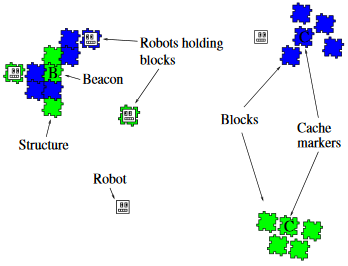
\includegraphics[width=\pictureWidthBig,keepaspectratio]{graphics/StrukturenKloetze.png}
%	\caption{Struktur-Erstellung mit Bausteinen}
%	\label{pic:StrukturenKloetze}
%\end{wrapfigure}

Mit einem anderen Ansatz ging man bei dem folgenden Paper an das Problem der Erstellung von Strukturen. Statt die Struktur mit den Robotern selbst aufzubauen, wurde sie stattdessen mit Bausteinen aufgebaut, die von Robotern zu ihrem Ort getragen wurde. Die Roboter selbst wurden dabei genau wie die Steine zufällig auf dem Gebiet ausgeworfen. Anschließend wurde ein Beacon erstellt, der die Position markiert, an der die entsprechende Struktur aufgebaut werden soll.

\begin{figure}[h]
	\centering
	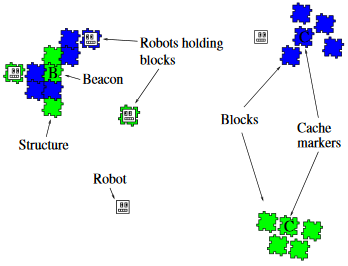
\includegraphics[width=0.8\textwidth,keepaspectratio]{graphics/StrukturenKloetze.png}
	\caption{Struktur-Erstellung mit Bausteinen}
	\label{pic:StrukturenKloetze}
\end{figure}

Die Roboter selbst können sich im 2dim-Feld in jede beliebige Richtung bewegen. Die Kommunikation der Roboter beschränkt sich darauf Kollisionen zu vermeiden. Das besondere an diesem Paper ist, dass die Roboter selbst nicht die Struktur kennen die gebaut werden soll, sondern die Bausteine. Diese werden von den Robotern getragen und teilen dann den Robotern mit, wenn sie sich an einem geeigneten Platz befinden um abgesetzt zu werden.\cite{RobotPatterns}
Der Aufbau ist in \autoref{pic:StrukturenKloetze} zu sehen.
